The social network and summarized text data is combined into a visualization that can be displayed in RShiny. The RShiny dashboard uses the packages visNetwork and igraph. visNetwork is an R package for visualizing networks that allows users to create dynamic and interactive visualizations. Users can physically manipulate edges and nodes in a network graph, select and view nodes by group, and customize the appearance of the network with colors and images. igraph is a set of fast and easy to use network analysis tools in R that allows the user to quickly set up and define network graph relationships that can then be ported over to visNetwork for visualization.

The visualizations were produced by combining the clustering results with the TextRank algorithm.
The clustering results output the set of nodes and their groupings. Then, the TextRank algorithm was applied to the communications between each set of nodes, reducing the large volumes of text for each pair of nodes to a single sentence that would in theory summarize their conversations. The Social Network Analysis results were similarly combined with the TextRank algorithm.

The code for producing these visualizations is included in the Appendices. Below are shown some screenshots of the visualizations when run in RStudio.

\begin{figure}[h]
	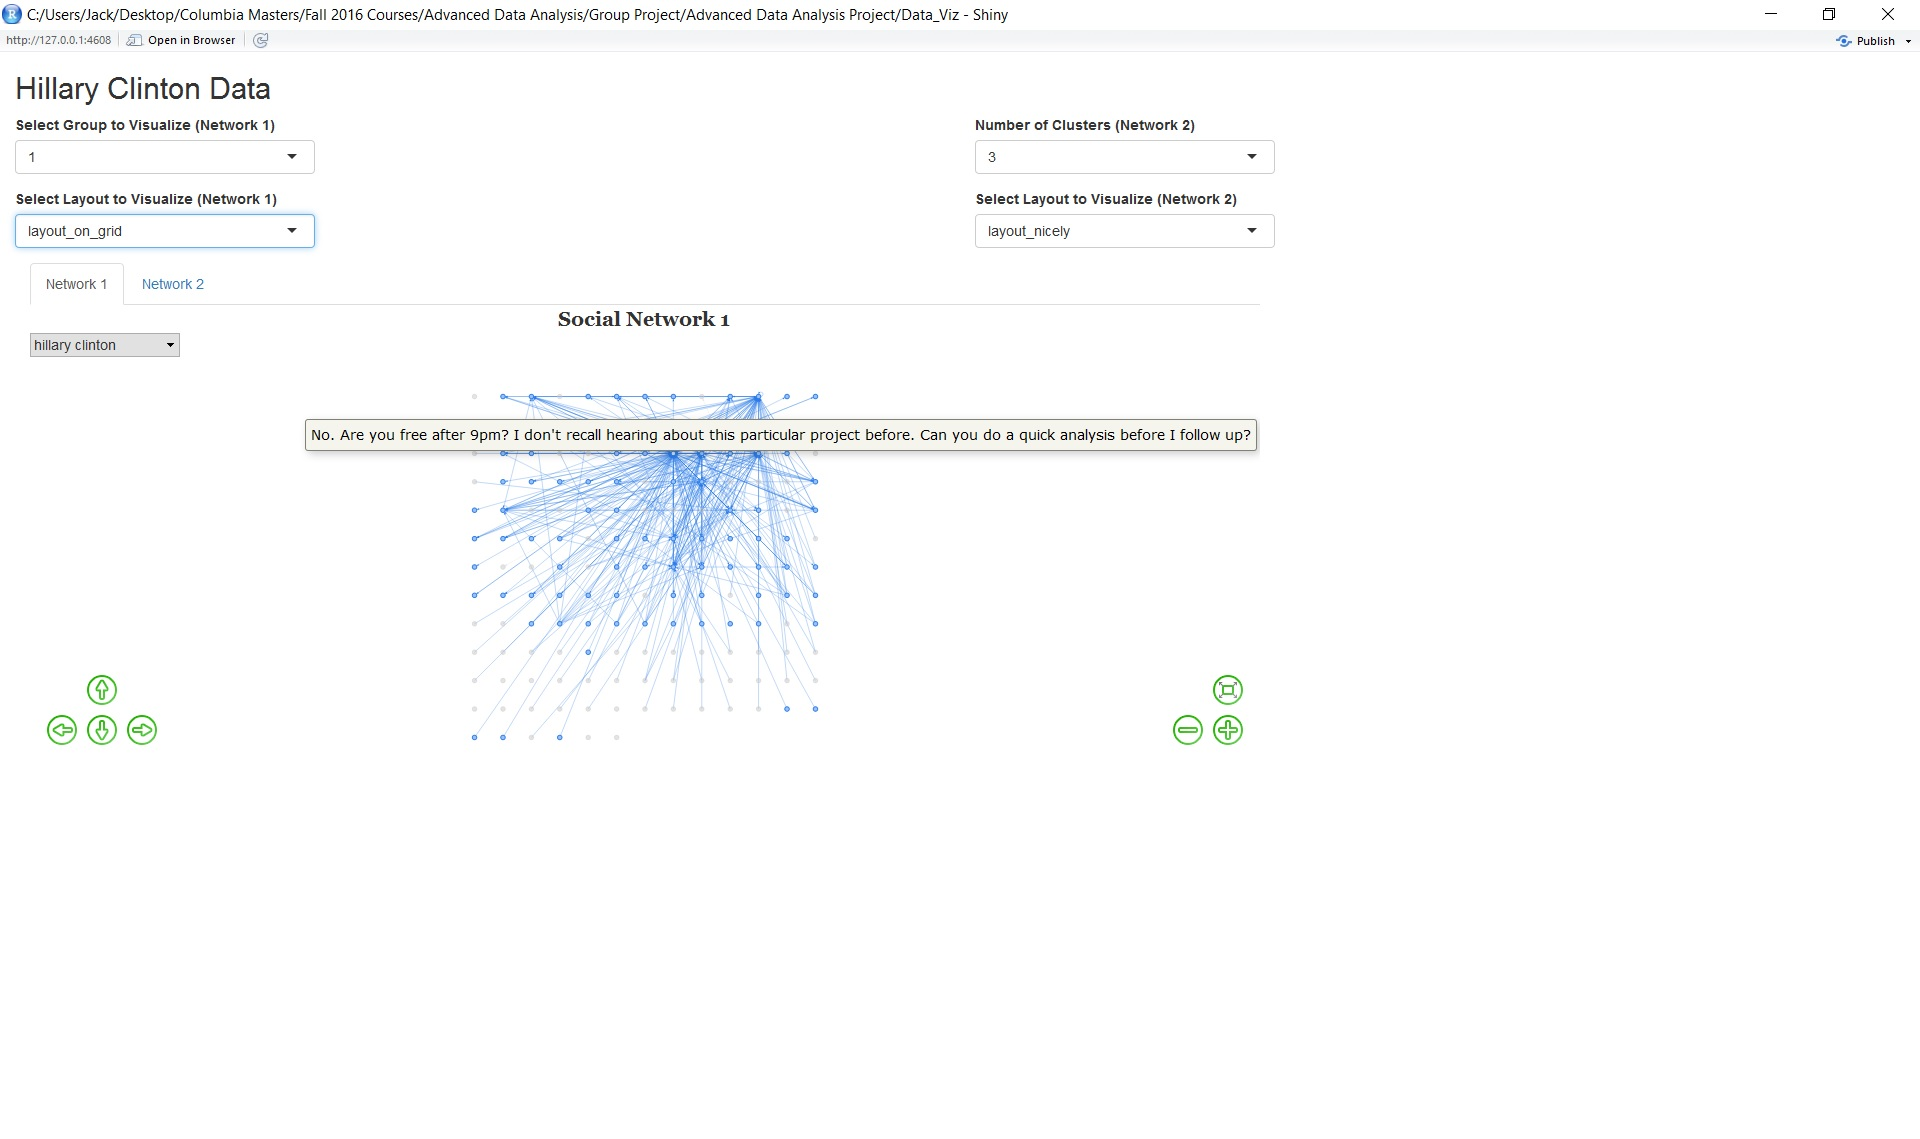
\includegraphics[width=10cm,height=10cm]{eric/Viz Screenshot 1}
	\caption{Insert caption}
	\label{Insert label}
\end{figure}

\begin{figure}[h]
	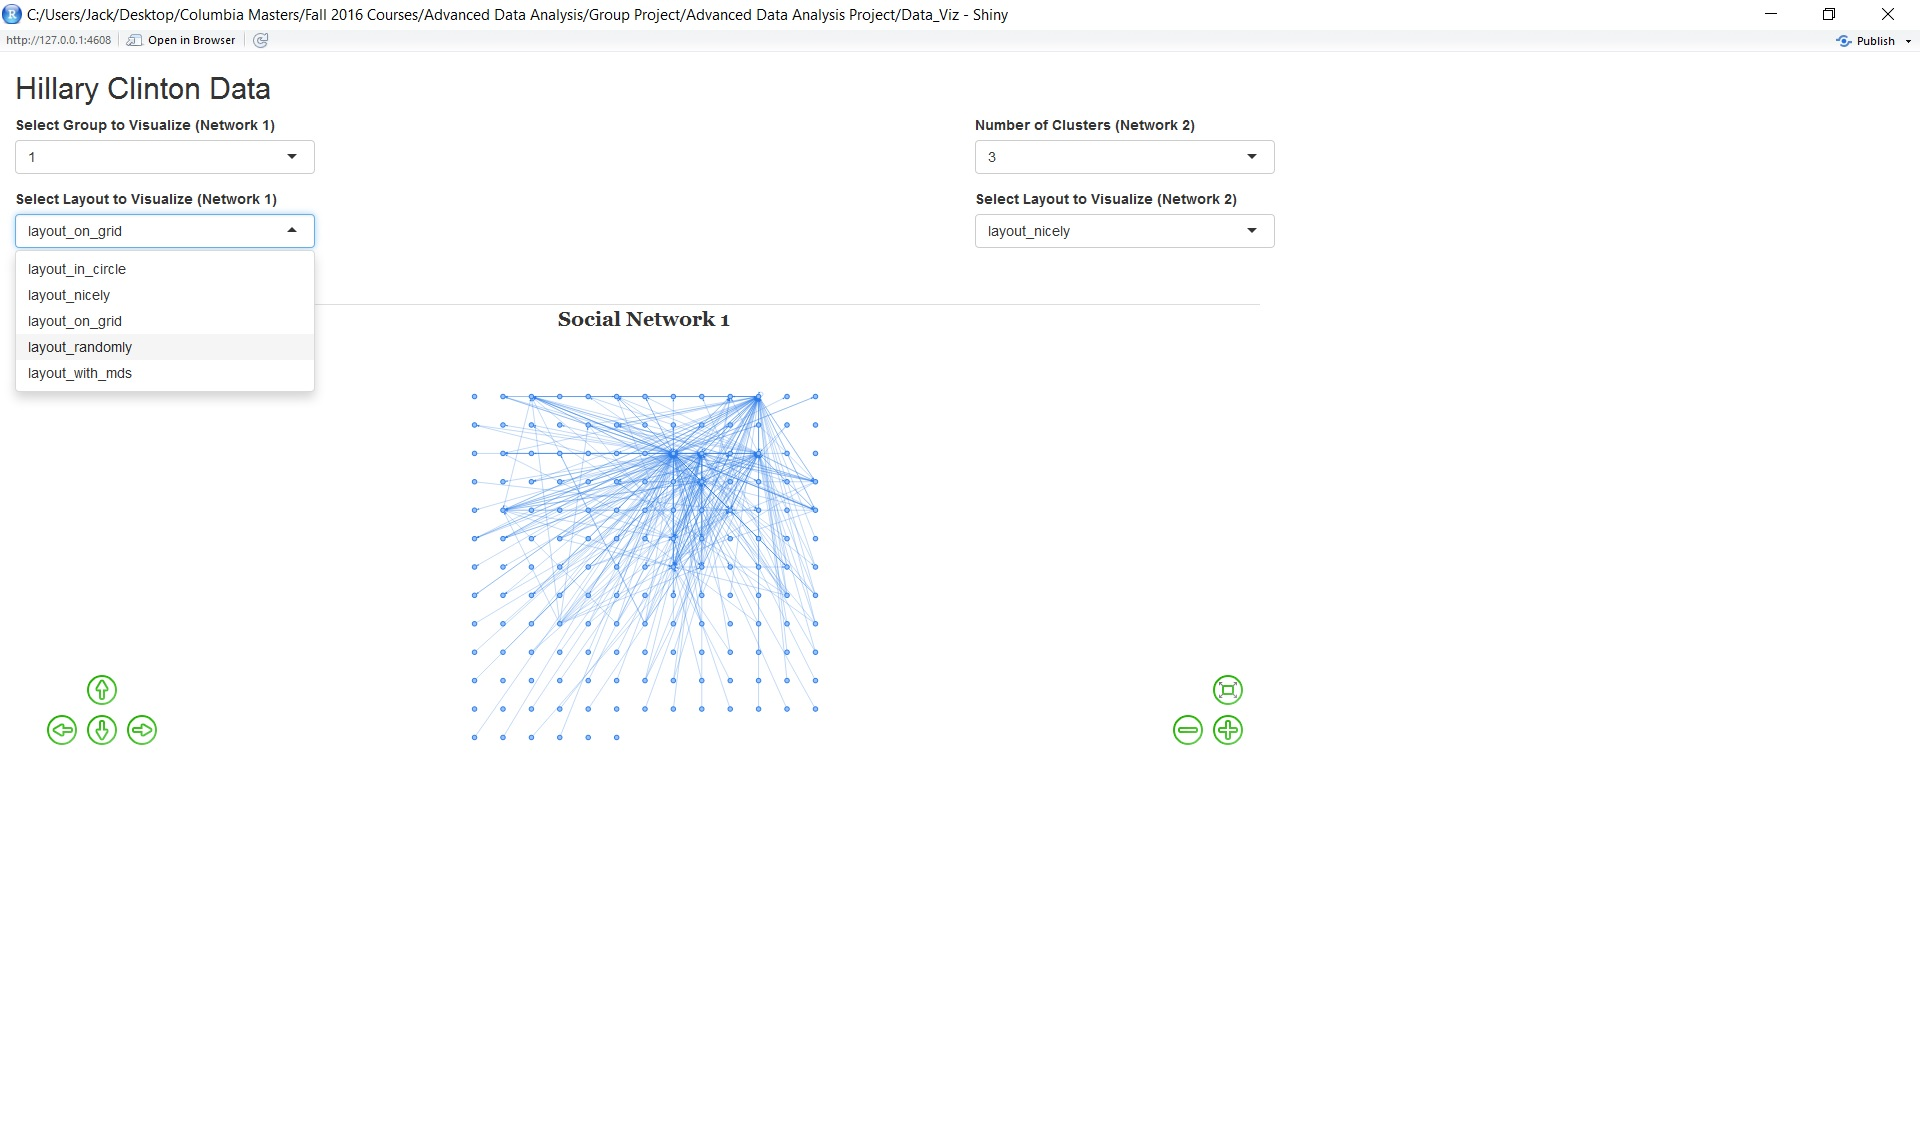
\includegraphics[width=10cm,height=10cm]{eric/Viz Screenshot 2}
	\caption{Insert caption}
	\label{Insert label}
\end{figure}

\begin{figure}[h]
	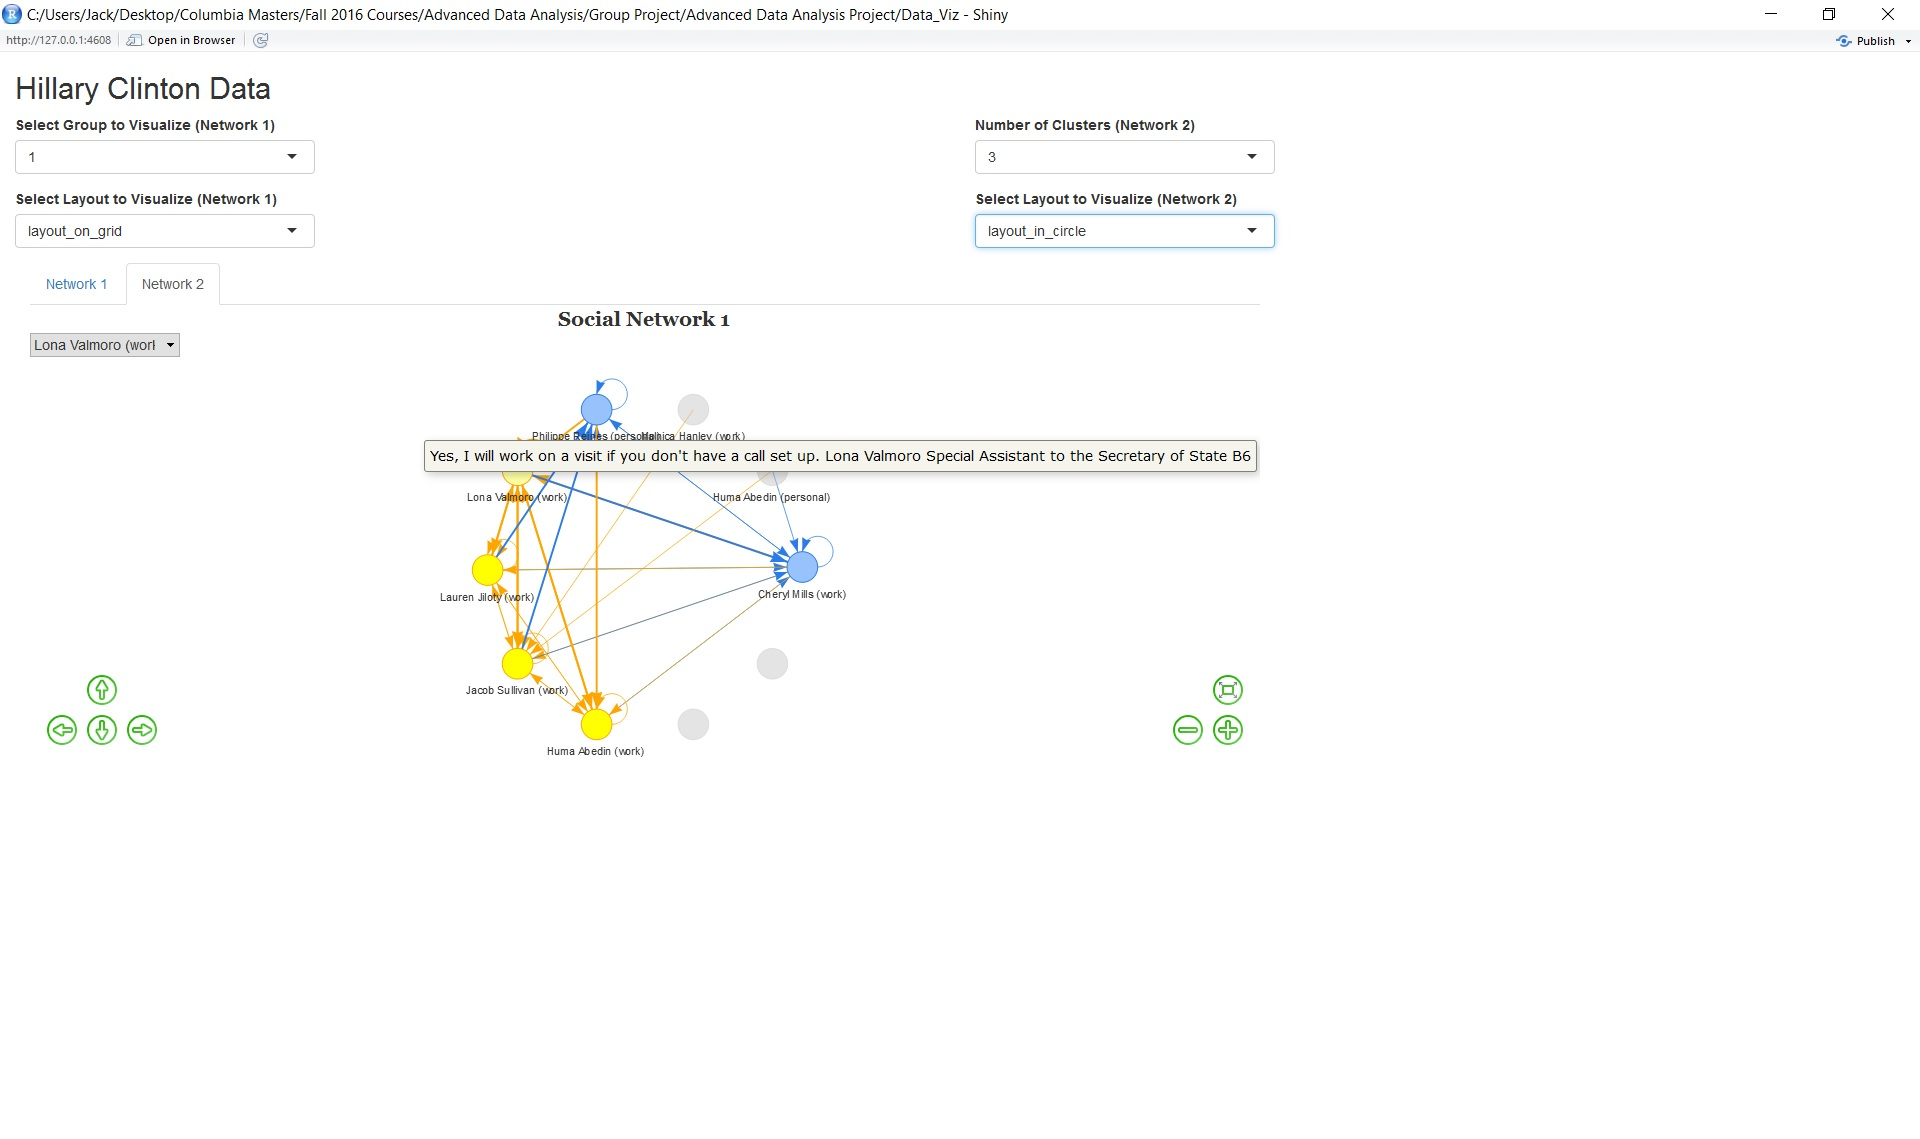
\includegraphics[width=10cm,height=10cm]{eric/Viz Screenshot 3}
	\caption{Insert caption}
	\label{Insert label}
\end{figure}

\begin{figure}[h]
	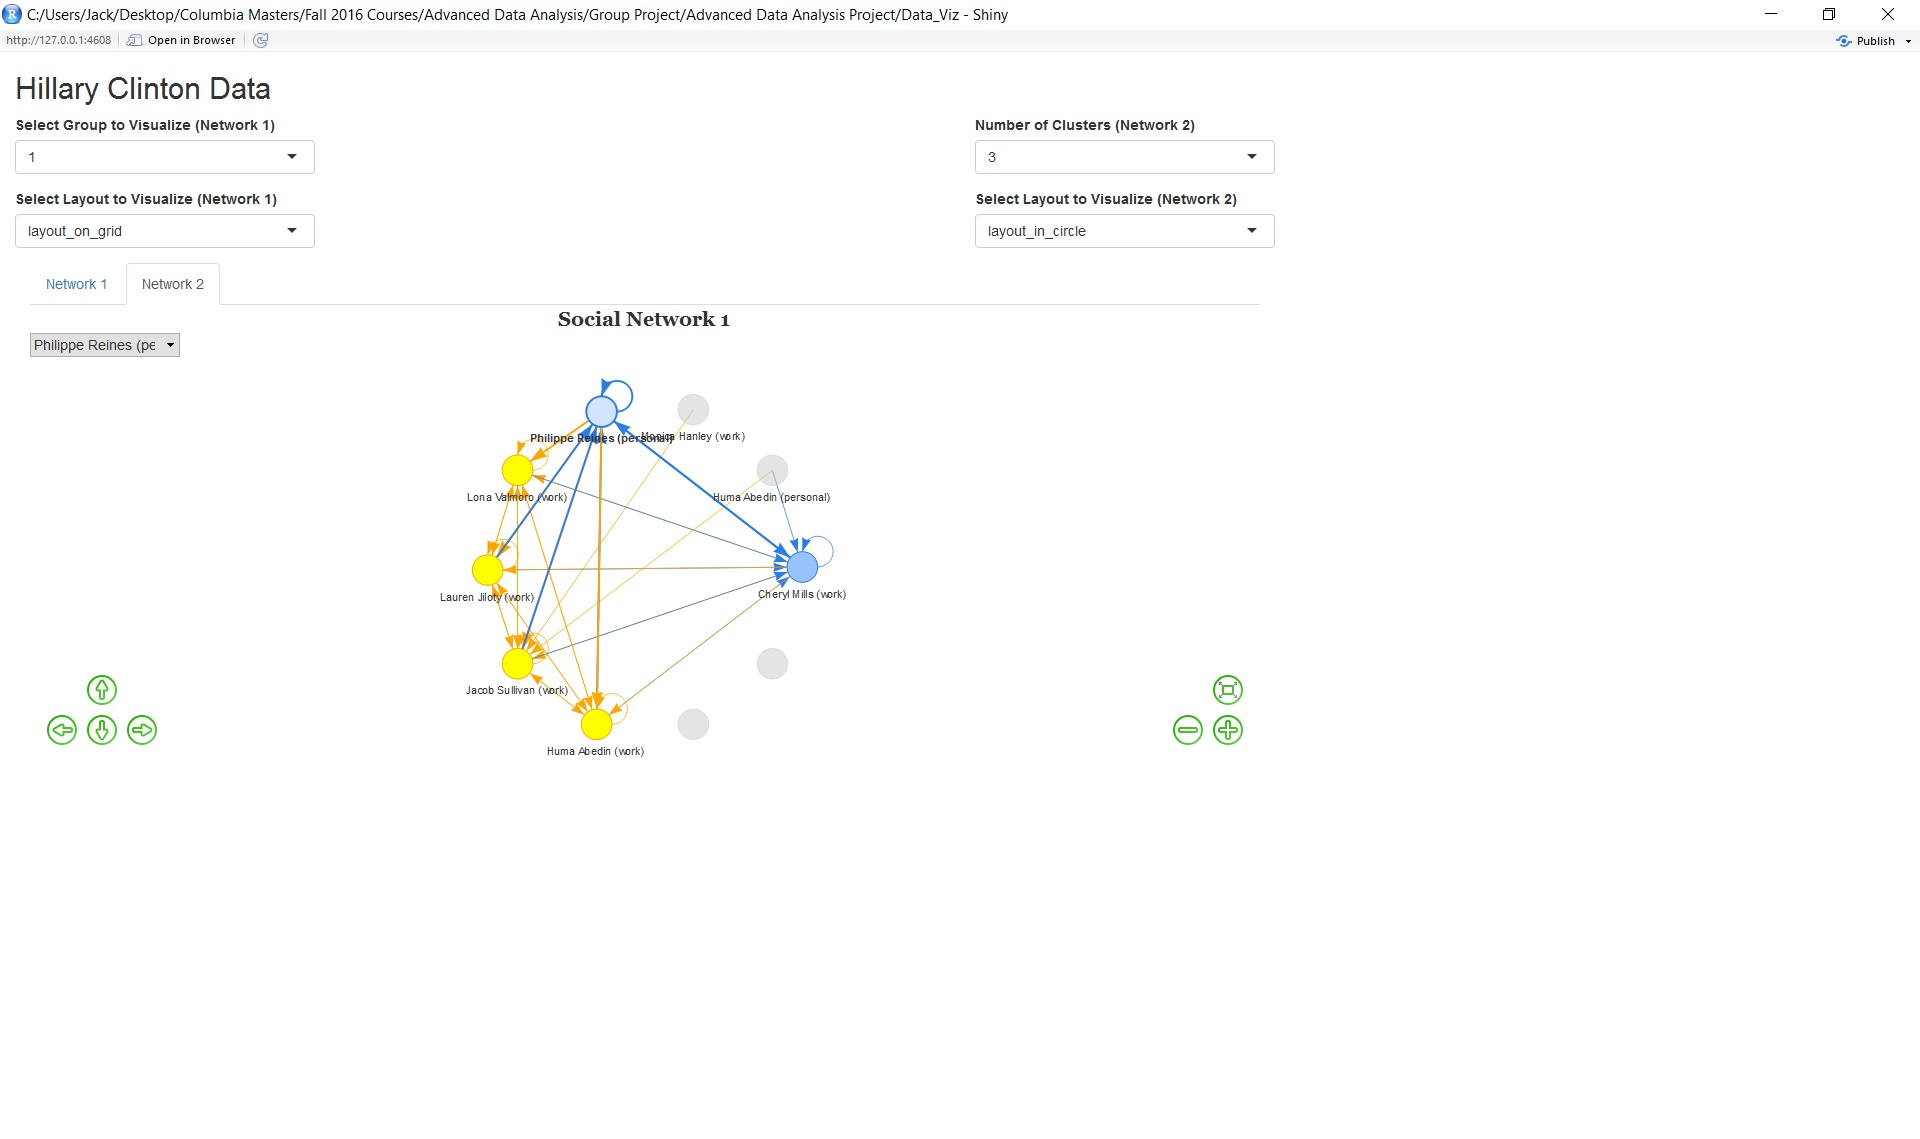
\includegraphics[width=10cm,height=10cm]{eric/Viz Screenshot 4}
	\caption{Insert caption}
	\label{Insert label}
\end{figure}
\end{document}